%
% File iscol2016.tex
%

\documentclass[11pt]{article}
\usepackage{acl-onecolumn}
\usepackage[margin=0.5in]{geometry}
\usepackage{times}
\usepackage{url}
\usepackage{amsmath}
\usepackage{breqn}
\usepackage{latexsym}
\usepackage{pgfplotstable}
\usepackage{algorithm2e}
\usepackage{hhline}
\usepackage{multirow}
\usepackage[font=footnotesize]{caption}
\usepackage{subcaption}
%\usepackage{hyperref}
\usepackage{color}
\usepackage{lipsum,adjustbox}
\usepackage{tikz}
\usepackage{tikz-dependency}
\usetikzlibrary{shapes,fit,calc,er,positioning,intersections,decorations.shapes,mindmap,trees}
\tikzset{decorate sep/.style 2 args={decorate,decoration={shape backgrounds,shape=circle,
      shape size=#1,shape sep=#2}}}

\setlength{\belowcaptionskip}{-10pt}
\newcommand{\secref}[1]{Section~\ref{#1}}
\newcommand{\figref}[1]{Figure~\ref{#1}}
\newcommand{\tabref}[1]{Table~\ref{#1}}

\makeatletter
\renewcommand{\paragraph}{
  \@startsection{paragraph}{4}
  {\z@}{.3ex \@plus .3ex \@minus .2ex}{-1em}
  {\normalfont\normalsize\bfseries}
}

\title{Broad-Coverage Semantic Parsing: A Transition-Based Approach}

\author{Daniel Hershcovich \and Omri Abend \and Ari Rappoport \\
  Institute of Computer Science \\
  Hebrew University of Jerusalem \\
  {\tt \{danielh,oabend,arir\}@cs.huji.ac.il}
}

\date{}


\begin{document}
\maketitle

\vspace{-2cm}
%%%%%%%%%%%%%%%%%%%%%%%%%%%%%%%%%%%%%%%%%%%%%%%%%%%%%%%%%%%%%%%
%%%%%%%%%%%%%%%%%     Abstract
%%%%%%%%%%%%%%%%%%%%%%%%%%%%%%%%%%%%%%%%%%%%%%%%%%%%%%%%%%%%%%%
\begin{abstract}

  The representation of many common semantic phenomena requires 
  structural properties beyond those commonly used for syntactic parsing.
  We discuss a set of structural properties required for
  broad-coverage semantic representation, and note that existing
  parsers support only some of these properties.
  We propose transition-based techniques for parsing such semantic structures:
  (1) conversion into related formalisms, and using existing parsers;
  and (2) a parser that directly supports the full set of properties.
  We experiment with UCCA-annotated corpora, the only ones with all these
  structural semantic properties. Results demonstrate the effectiveness
  of transition-based methods for the task.
  
\end{abstract}



%%%%%%%%%%%%%%%%%%%%%%%%%%%%%%%%%%%%%%%%%%%%%%%%%%%%%%%%%%%%%%%
\section{Introduction}

To represent the full range of semantic structures exhibited by
natural language, three structural properties should be supported.
The first is \textbf{multiple parents},
representing arguments and relations (semantic units) that are shared between predicates.
For instance, in \figref{fig:graduation}, ``John'' is an argument of both ``graduation''
and ``moved'', yielding a DAG structure rather than a tree.
The second is \textbf{non-terminal nodes} for representing units
comprising more than one word.
While bi-lexical dependencies partially circumvent this
using headwords, they fall short when representing units that have no clear head,
such as the coordination structure in \figref{fig:home}.
Third, semantic units may be \textbf{discontinuous}.
For instance, the phrasal verb ``gave ... up'' in \figref{fig:gave} forms a single semantic unit.
We call formal representations supporting all three properties 
{\it Broad-coverage Semantic Structures} (BSS).

\begin{figure}[ht]
  \begin{subfigure}[ht]{.43\textwidth}
  \scalebox{.8}{
  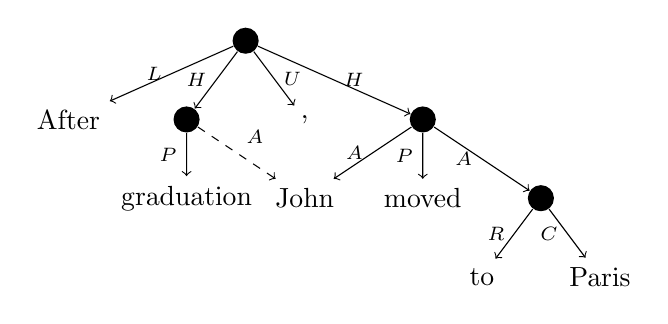
\begin{tikzpicture}[level distance=10mm, ->]
    \node (ROOT) [fill=black, circle] {}
      child {node (After) {After} edge from parent node[left] {\scriptsize $L$}}
      child {node (graduation) [fill=black, circle] {}
      {
        child {node {graduation} edge from parent node[left] {\scriptsize $P$}}
      } edge from parent node[left] {\scriptsize $H$} }
      child {node {,} edge from parent node[right] {\scriptsize $U$}}
      child {node (moved) [fill=black, circle] {}
      {
        child {node (John) {John} edge from parent node[left] {\scriptsize $A$}}
        child {node {moved} edge from parent node[left] {\scriptsize $P$}}
        child {node [fill=black, circle] {}
        {
          child {node {to} edge from parent node[left] {\scriptsize $R$}}
          child {node {Paris} edge from parent node[left] {\scriptsize $C$}}
        } edge from parent node[left] {\scriptsize $A$} }
      } edge from parent node[right] {\scriptsize $H$} }
      ;
    \draw[dashed,->] (graduation) to node [auto] {\scriptsize $A$} (John);
  \end{tikzpicture}
  }
  \caption{}\label{fig:graduation}
  \end{subfigure}
  \begin{subfigure}[ht]{.33\textwidth}
  \scalebox{.91}{
  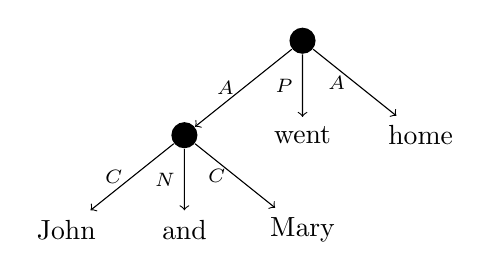
\begin{tikzpicture}[level distance=12mm, ->,
      every node/.append style={midway}]
    \node (ROOT) [fill=black, circle] {}
      child {node [fill=black, circle] {}
      {
        child {node {John} edge from parent node[left] {\scriptsize $C$}}
        child {node {and} edge from parent node[left] {\scriptsize $N$}}
        child {node {Mary} edge from parent node[left] {\scriptsize $C$}}
      } edge from parent node[left] {\scriptsize $A$} }
      child {node {went} edge from parent node[left] {\scriptsize $P$}}
      child {node {home} edge from parent node[left] {\scriptsize $A$}}
      ;
  \end{tikzpicture}
  }
  \caption{}\label{fig:home}
  \end{subfigure}
  \begin{subfigure}[ht]{.23\textwidth}
  \scalebox{.91}{
  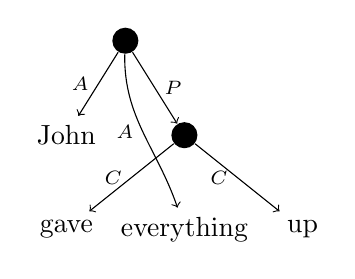
\begin{tikzpicture}[level distance=12mm, ->,
      every node/.append style={midway}]
    \node (ROOT) [fill=black, circle] {}
      child {node {John} edge from parent node[left] {\scriptsize $A$}}
      child {node [fill=black, circle] {}
      {
      	child {node {gave} edge from parent node[left] {\scriptsize $C$}}
      	child {node (everything) {everything} edge from parent[white]}
      	child {node {up} edge from parent node[left] {\scriptsize $C$}}
      } edge from parent node[right] {\scriptsize $P$} }
      ;
    \draw[bend right,->] (ROOT) to[out=-20, in=180] node [left] {\scriptsize $A$} (everything);
  \end{tikzpicture}
  }
  \caption{}\label{fig:gave}
  \end{subfigure}
  \caption{\label{fig:examples}\footnotesize
    Semantic representation of the three structural properties
    required for BSS, according to the UCCA scheme. (\subref{fig:graduation}) includes a remote edge (dashed),
    resulting in ``John'' having two parents.
    (\subref{fig:home}) includes a coordination construction.
    (\subref{fig:gave}) includes a discontinuous unit.
    Legend: $P$ -- a Scene's main relation, $A$ -- participant,
    $L$ -- inter-scene linker, $H$ -- linked Scene, $C$ -- center,
    $R$ -- relator, $N$ -- connector, $U$ -- punctuation.
    Pre-terminal nodes are omitted for brevity.
  }
\end{figure}

No existing parser supports the combination of these criteria.
The only semantic annotation scheme that supports them is UCCA \cite{abend2013universal}.
Several other models support only some of them \cite{oepen2015semeval},
or avoid grounding semantic units altogether \cite{banarescu2013abstract}.

We are first in proposing techniques for BSS parsing.
We adopt a transition-based approach, which has recently produced some of the best
results in dependency parsing \cite{dyer2015transition}.
This is a natural starting point for parsing UCCA, as
the set of distinctions it represents, centered around predicate-argument
structures and their inter-relations, is similar in spirit to the distinctions
conveyed by dependency schemes.


%%%%%%%%%%%%%%%%%%%%%%%%%%%%%%%%%%%%%%%%%%%%%%%%%%%%%%%%%%%%%%%
\section{Conversion-Based Parsing}\label{sec:conversion_approach}

We convert BSS into a representation compatible with existing parsers,
and train the parsers on the converted structures.
We evaluate the trained parsers by applying them to the test set,
and converting the results back to BSS, where they are compared
with the gold standard.

\paragraph{Conversion to Constituency Trees.}
We convert BSS to constituency trees by removing a subset of the
edges.
Specifically, when converting UCCA structures, we remove all remote edges,
leaving only primary edges, which form a tree structure (see \figref{fig:graduation}).
The inverse conversion is simply the identity function.

\paragraph{Conversion to Dependency Trees.}\label{subsec:con2dep}
After obtaining constituency trees, we remove
all non-terminals and add edges between terminals.
The inverse conversion introduces non-terminal nodes back into the tree.
Edge labels for intermediate edges introduced in the conversion are determined by a rule-based function.



%%%%%%%%%%%%%%%%%%%%%%%%%%%%%%%%%%%%%%%%%%%%%%%%%%%%%%%%%%%%%%%
\section{Broad-Coverage Semantic Parsing}\label{sec:direct_approach}

We present \textsc{bsp}, a transition-based parser supporting the three BSS criteria.
We build on recent advances in discontinuous constituency
and dependency DAG parsing, and introduce novel features for parsing BSS.

\paragraph{Transition Set.}
In addition to the standard transitions in shift-reduce parsing, 
we include transitions for creating non-terminal nodes \cite{sagae2005classifier},
for creating primary and remote edges,
and for discontinuous parsing \cite{maier2015discontinuous}.
As in other work on
transition-based DAG dependency parsing \cite{sagae2008shift},
node and edge transitions do not pop the stack,
to support multiple parents.

\paragraph{Classifier.}
We train an averaged structured perceptron
\cite{Coll:04} with \textsc{MinUpdate} \cite{goldberg2011learning} and
a dynamic oracle \cite{goldberg2012dynamic}.
Inference is performed greedily.


%%%%%%%%%%%%%%%%%%%%%%%%%%%%%%%%%%%%%%%%%%%%%%%%%%%%%%%%%%%%%%%
\section{Experimentals}\label{sec:experiments}

\paragraph{Data.}\label{sec:data}
We conduct our experiments on the UCCA Wikipedia corpus (\textit{Wiki}),
and use the English part of the UCCA \textit{Twenty Thousand Leagues Under the Sea} English-French parallel corpus as
out-of-domain data.\footnote{Both are available at \url{http://www.cs.huji.ac.il/~oabend/ucca.html}}

\paragraph{Conversions.}
We parse converted constituency trees with \textsc{uparse},
and converted dependency trees with MaltParser \cite{nivre2007maltparser}
and the stack LSTM-based parser \cite{dyer2015transition}.

\paragraph{Results.}
\tabref{table:results} presents our experimental results.
The LSTM parser obtains the highest primary F-score, with a considerable margin.
This suggests that a similar classifier is likely to improve results for \textsc{bsp}.

\begin{table}[ht]
\centering
\begin{subtable}{.4\textwidth}
\scalebox{.8}{
\begin{tabular}{l|ccc|ccc}
& \multicolumn{3}{c|}{\footnotesize Primary} & \multicolumn{3}{c}{\footnotesize Remote} \\
& \textbf{LP} & \textbf{LR} & \textbf{LF} & \textbf{LP} & \textbf{LR} & \textbf{LF} \\
\hline
\multicolumn{4}{l}{\rule{0pt}{2ex} \footnotesize Constituency Tree Conversion} \\
\textsc{uparse} & 64 & 67.3 & 65.4 & $-$ & 0 & 0 \\
Upper Bound & 100 & 100 & 100 & $-$ & 0 & 0 \\
\hline
\multicolumn{4}{l}{\rule{0pt}{3ex} \footnotesize Dependency Tree Conversion} \\
Malt$_{\textrm{arc-eager}}$ & 63.9 & 57.9 & 60.5 & $-$ & 0 & 0 \\
LSTM & {\bf 73.2} & {\bf 66.2} & {\bf 69.2} & $-$ & 0 & 0 \\
Upper Bound & 93.8 & 83.7 & 88.4 & $-$ & 0 & 0
\end{tabular}
}
\caption{\label{table:conversion_results}}
\end{subtable}
\hspace{.1\textwidth}
\begin{subtable}{.4\textwidth}
\scalebox{.8}{
\begin{tabular}{l|ccc|ccc}
& \multicolumn{3}{c|}{\footnotesize Primary} & \multicolumn{3}{c}{\footnotesize Remote} \\
& \textbf{LP} & \textbf{LR} & \textbf{LF} & \textbf{LP} & \textbf{LR} & \textbf{LF} \\
\hline
\multicolumn{4}{l}{\rule{0pt}{2ex} \footnotesize In-domain} \\
\textsc{bsp} & 62.4 & 56 & 59 & 15.3 & 11.8 & 13.3 \\
\textsc{bsp}$_{\mathrm{Tree}}$ & 63.8 & 56.5 & 59.9 & $-$ & 0 & 0 \\
\hline
\multicolumn{4}{l}{\rule{0pt}{3ex} \footnotesize Out-of-domain} \\
\textsc{bsp} & 60.6 & 53.9 & 57.1 & 20.2 & 10.3 & 13.6 \\
\textsc{bsp}$_{\mathrm{Tree}}$ & 60.2 & 52.8 & 56.2 & $-$ & 0 & 0
\end{tabular}
}
\caption{\label{table:bsp_results}}
\end{subtable}
\caption{\footnotesize
  Main experimental results in percents.
  (a) Results on the \textit{Wiki} test set
  after conversion to constituency trees (top) and dependency trees (bottom).
  (b) Results on the \textit{Wiki} test set (top) and on out-of-domain data (bottom)
  for our \textsc{bsp}, when trained on UCCA DAGs (\textsc{bsp}),
  and when trained on trees obtained by removing remote edges (\textsc{bsp}$_{\mathrm{Tree}}$).
}
\label{table:results}
\end{table}


\bibliography{references}
\bibliographystyle{acl2016}

\end{document}
